\documentclass[11pt,preprint, authoryear]{elsarticle}

\usepackage{lmodern}
%%%% My spacing
\usepackage{setspace}
\setstretch{1.2}
\DeclareMathSizes{12}{14}{10}{10}

% Wrap around which gives all figures included the [H] command, or places it "here". This can be tedious to code in Rmarkdown.
\usepackage{float}
\let\origfigure\figure
\let\endorigfigure\endfigure
\renewenvironment{figure}[1][2] {
    \expandafter\origfigure\expandafter[H]
} {
    \endorigfigure
}

\let\origtable\table
\let\endorigtable\endtable
\renewenvironment{table}[1][2] {
    \expandafter\origtable\expandafter[H]
} {
    \endorigtable
}


\usepackage{ifxetex,ifluatex}
\usepackage{fixltx2e} % provides \textsubscript
\ifnum 0\ifxetex 1\fi\ifluatex 1\fi=0 % if pdftex
  \usepackage[T1]{fontenc}
  \usepackage[utf8]{inputenc}
\else % if luatex or xelatex
  \ifxetex
    \usepackage{mathspec}
    \usepackage{xltxtra,xunicode}
  \else
    \usepackage{fontspec}
  \fi
  \defaultfontfeatures{Mapping=tex-text,Scale=MatchLowercase}
  \newcommand{\euro}{€}
\fi

\usepackage{amssymb, amsmath, amsthm, amsfonts}

\def\bibsection{\section*{References}} %%% Make "References" appear before bibliography


\usepackage[round]{natbib}

\usepackage{longtable}
\usepackage[margin=2.3cm,bottom=2cm,top=2.5cm, includefoot]{geometry}
\usepackage{fancyhdr}
\usepackage[bottom, hang, flushmargin]{footmisc}
\usepackage{graphicx}
\numberwithin{equation}{section}
\numberwithin{figure}{section}
\numberwithin{table}{section}
\setlength{\parindent}{0cm}
\setlength{\parskip}{1.3ex plus 0.5ex minus 0.3ex}
\usepackage{textcomp}
\renewcommand{\headrulewidth}{0.2pt}
\renewcommand{\footrulewidth}{0.3pt}

\usepackage{array}
\newcolumntype{x}[1]{>{\centering\arraybackslash\hspace{0pt}}p{#1}}

%%%%  Remove the "preprint submitted to" part. Don't worry about this either, it just looks better without it:
\makeatletter
\def\ps@pprintTitle{%
  \let\@oddhead\@empty
  \let\@evenhead\@empty
  \let\@oddfoot\@empty
  \let\@evenfoot\@oddfoot
}
\makeatother

 \def\tightlist{} % This allows for subbullets!

\usepackage{hyperref}
\hypersetup{breaklinks=true,
            bookmarks=true,
            colorlinks=true,
            citecolor=blue,
            urlcolor=blue,
            linkcolor=blue,
            pdfborder={0 0 0}}


% The following packages allow huxtable to work:
\usepackage{siunitx}
\usepackage{multirow}
\usepackage{hhline}
\usepackage{calc}
\usepackage{tabularx}
\usepackage{booktabs}
\usepackage{caption}


\newenvironment{columns}[1][]{}{}

\newenvironment{column}[1]{\begin{minipage}{#1}\ignorespaces}{%
\end{minipage}
\ifhmode\unskip\fi
\aftergroup\useignorespacesandallpars}

\def\useignorespacesandallpars#1\ignorespaces\fi{%
#1\fi\ignorespacesandallpars}

\makeatletter
\def\ignorespacesandallpars{%
  \@ifnextchar\par
    {\expandafter\ignorespacesandallpars\@gobble}%
    {}%
}
\makeatother

\newlength{\cslhangindent}
\setlength{\cslhangindent}{1.5em}
\newenvironment{CSLReferences}%
  {\setlength{\parindent}{0pt}%
  \everypar{\setlength{\hangindent}{\cslhangindent}}\ignorespaces}%
  {\par}


\urlstyle{same}  % don't use monospace font for urls
\setlength{\parindent}{0pt}
\setlength{\parskip}{6pt plus 2pt minus 1pt}
\setlength{\emergencystretch}{3em}  % prevent overfull lines
\setcounter{secnumdepth}{5}

%%% Use protect on footnotes to avoid problems with footnotes in titles
\let\rmarkdownfootnote\footnote%
\def\footnote{\protect\rmarkdownfootnote}
\IfFileExists{upquote.sty}{\usepackage{upquote}}{}

%%% Include extra packages specified by user
\usepackage{booktabs}
\usepackage{longtable}
\usepackage{array}
\usepackage{multirow}
\usepackage{wrapfig}
\usepackage{float}
\usepackage{colortbl}
\usepackage{pdflscape}
\usepackage{tabu}
\usepackage{threeparttable}
\usepackage{threeparttablex}
\usepackage[normalem]{ulem}
\usepackage{makecell}
\usepackage{xcolor}
\usepackage{caption}
\usepackage{graphicx}
\usepackage{siunitx}
\usepackage{hhline}
\usepackage{calc}
\usepackage{tabularx}
\usepackage{adjustbox}
\usepackage{hyperref}

%%% Hard setting column skips for reports - this ensures greater consistency and control over the length settings in the document.
%% page layout
%% paragraphs
\setlength{\baselineskip}{12pt plus 0pt minus 0pt}
\setlength{\parskip}{12pt plus 0pt minus 0pt}
\setlength{\parindent}{0pt plus 0pt minus 0pt}
%% floats
\setlength{\floatsep}{12pt plus 0 pt minus 0pt}
\setlength{\textfloatsep}{20pt plus 0pt minus 0pt}
\setlength{\intextsep}{14pt plus 0pt minus 0pt}
\setlength{\dbltextfloatsep}{20pt plus 0pt minus 0pt}
\setlength{\dblfloatsep}{14pt plus 0pt minus 0pt}
%% maths
\setlength{\abovedisplayskip}{12pt plus 0pt minus 0pt}
\setlength{\belowdisplayskip}{12pt plus 0pt minus 0pt}
%% lists
\setlength{\topsep}{10pt plus 0pt minus 0pt}
\setlength{\partopsep}{3pt plus 0pt minus 0pt}
\setlength{\itemsep}{5pt plus 0pt minus 0pt}
\setlength{\labelsep}{8mm plus 0mm minus 0mm}
\setlength{\parsep}{\the\parskip}
\setlength{\listparindent}{\the\parindent}
%% verbatim
\setlength{\fboxsep}{5pt plus 0pt minus 0pt}


\usepackage{color}
\usepackage{fancyvrb}
\newcommand{\VerbBar}{|}
\newcommand{\VERB}{\Verb[commandchars=\\\{\}]}
\DefineVerbatimEnvironment{Highlighting}{Verbatim}{commandchars=\\\{\}}
% Add ',fontsize=\small' for more characters per line
\usepackage{framed}
\definecolor{shadecolor}{RGB}{248,248,248}
\newenvironment{Shaded}{\begin{snugshade}}{\end{snugshade}}
\newcommand{\AlertTok}[1]{\textcolor[rgb]{0.94,0.16,0.16}{#1}}
\newcommand{\AnnotationTok}[1]{\textcolor[rgb]{0.56,0.35,0.01}{\textbf{\textit{#1}}}}
\newcommand{\AttributeTok}[1]{\textcolor[rgb]{0.77,0.63,0.00}{#1}}
\newcommand{\BaseNTok}[1]{\textcolor[rgb]{0.00,0.00,0.81}{#1}}
\newcommand{\BuiltInTok}[1]{#1}
\newcommand{\CharTok}[1]{\textcolor[rgb]{0.31,0.60,0.02}{#1}}
\newcommand{\CommentTok}[1]{\textcolor[rgb]{0.56,0.35,0.01}{\textit{#1}}}
\newcommand{\CommentVarTok}[1]{\textcolor[rgb]{0.56,0.35,0.01}{\textbf{\textit{#1}}}}
\newcommand{\ConstantTok}[1]{\textcolor[rgb]{0.00,0.00,0.00}{#1}}
\newcommand{\ControlFlowTok}[1]{\textcolor[rgb]{0.13,0.29,0.53}{\textbf{#1}}}
\newcommand{\DataTypeTok}[1]{\textcolor[rgb]{0.13,0.29,0.53}{#1}}
\newcommand{\DecValTok}[1]{\textcolor[rgb]{0.00,0.00,0.81}{#1}}
\newcommand{\DocumentationTok}[1]{\textcolor[rgb]{0.56,0.35,0.01}{\textbf{\textit{#1}}}}
\newcommand{\ErrorTok}[1]{\textcolor[rgb]{0.64,0.00,0.00}{\textbf{#1}}}
\newcommand{\ExtensionTok}[1]{#1}
\newcommand{\FloatTok}[1]{\textcolor[rgb]{0.00,0.00,0.81}{#1}}
\newcommand{\FunctionTok}[1]{\textcolor[rgb]{0.00,0.00,0.00}{#1}}
\newcommand{\ImportTok}[1]{#1}
\newcommand{\InformationTok}[1]{\textcolor[rgb]{0.56,0.35,0.01}{\textbf{\textit{#1}}}}
\newcommand{\KeywordTok}[1]{\textcolor[rgb]{0.13,0.29,0.53}{\textbf{#1}}}
\newcommand{\NormalTok}[1]{#1}
\newcommand{\OperatorTok}[1]{\textcolor[rgb]{0.81,0.36,0.00}{\textbf{#1}}}
\newcommand{\OtherTok}[1]{\textcolor[rgb]{0.56,0.35,0.01}{#1}}
\newcommand{\PreprocessorTok}[1]{\textcolor[rgb]{0.56,0.35,0.01}{\textit{#1}}}
\newcommand{\RegionMarkerTok}[1]{#1}
\newcommand{\SpecialCharTok}[1]{\textcolor[rgb]{0.00,0.00,0.00}{#1}}
\newcommand{\SpecialStringTok}[1]{\textcolor[rgb]{0.31,0.60,0.02}{#1}}
\newcommand{\StringTok}[1]{\textcolor[rgb]{0.31,0.60,0.02}{#1}}
\newcommand{\VariableTok}[1]{\textcolor[rgb]{0.00,0.00,0.00}{#1}}
\newcommand{\VerbatimStringTok}[1]{\textcolor[rgb]{0.31,0.60,0.02}{#1}}
\newcommand{\WarningTok}[1]{\textcolor[rgb]{0.56,0.35,0.01}{\textbf{\textit{#1}}}}

\begin{document}



%titlepage
\thispagestyle{empty}
\begin{center}
\begin{minipage}{0.75\linewidth}
    \centering
%Entry1
    {\uppercase{\huge Exploring Machine Learning: Predicting Income and
Race\par}}
    \vspace{2cm}
%Author's name
    {\LARGE Cassandra Pengelly \textbar{} 20346212\par}
    \vspace{1cm}
%University logo
\begin{center}
    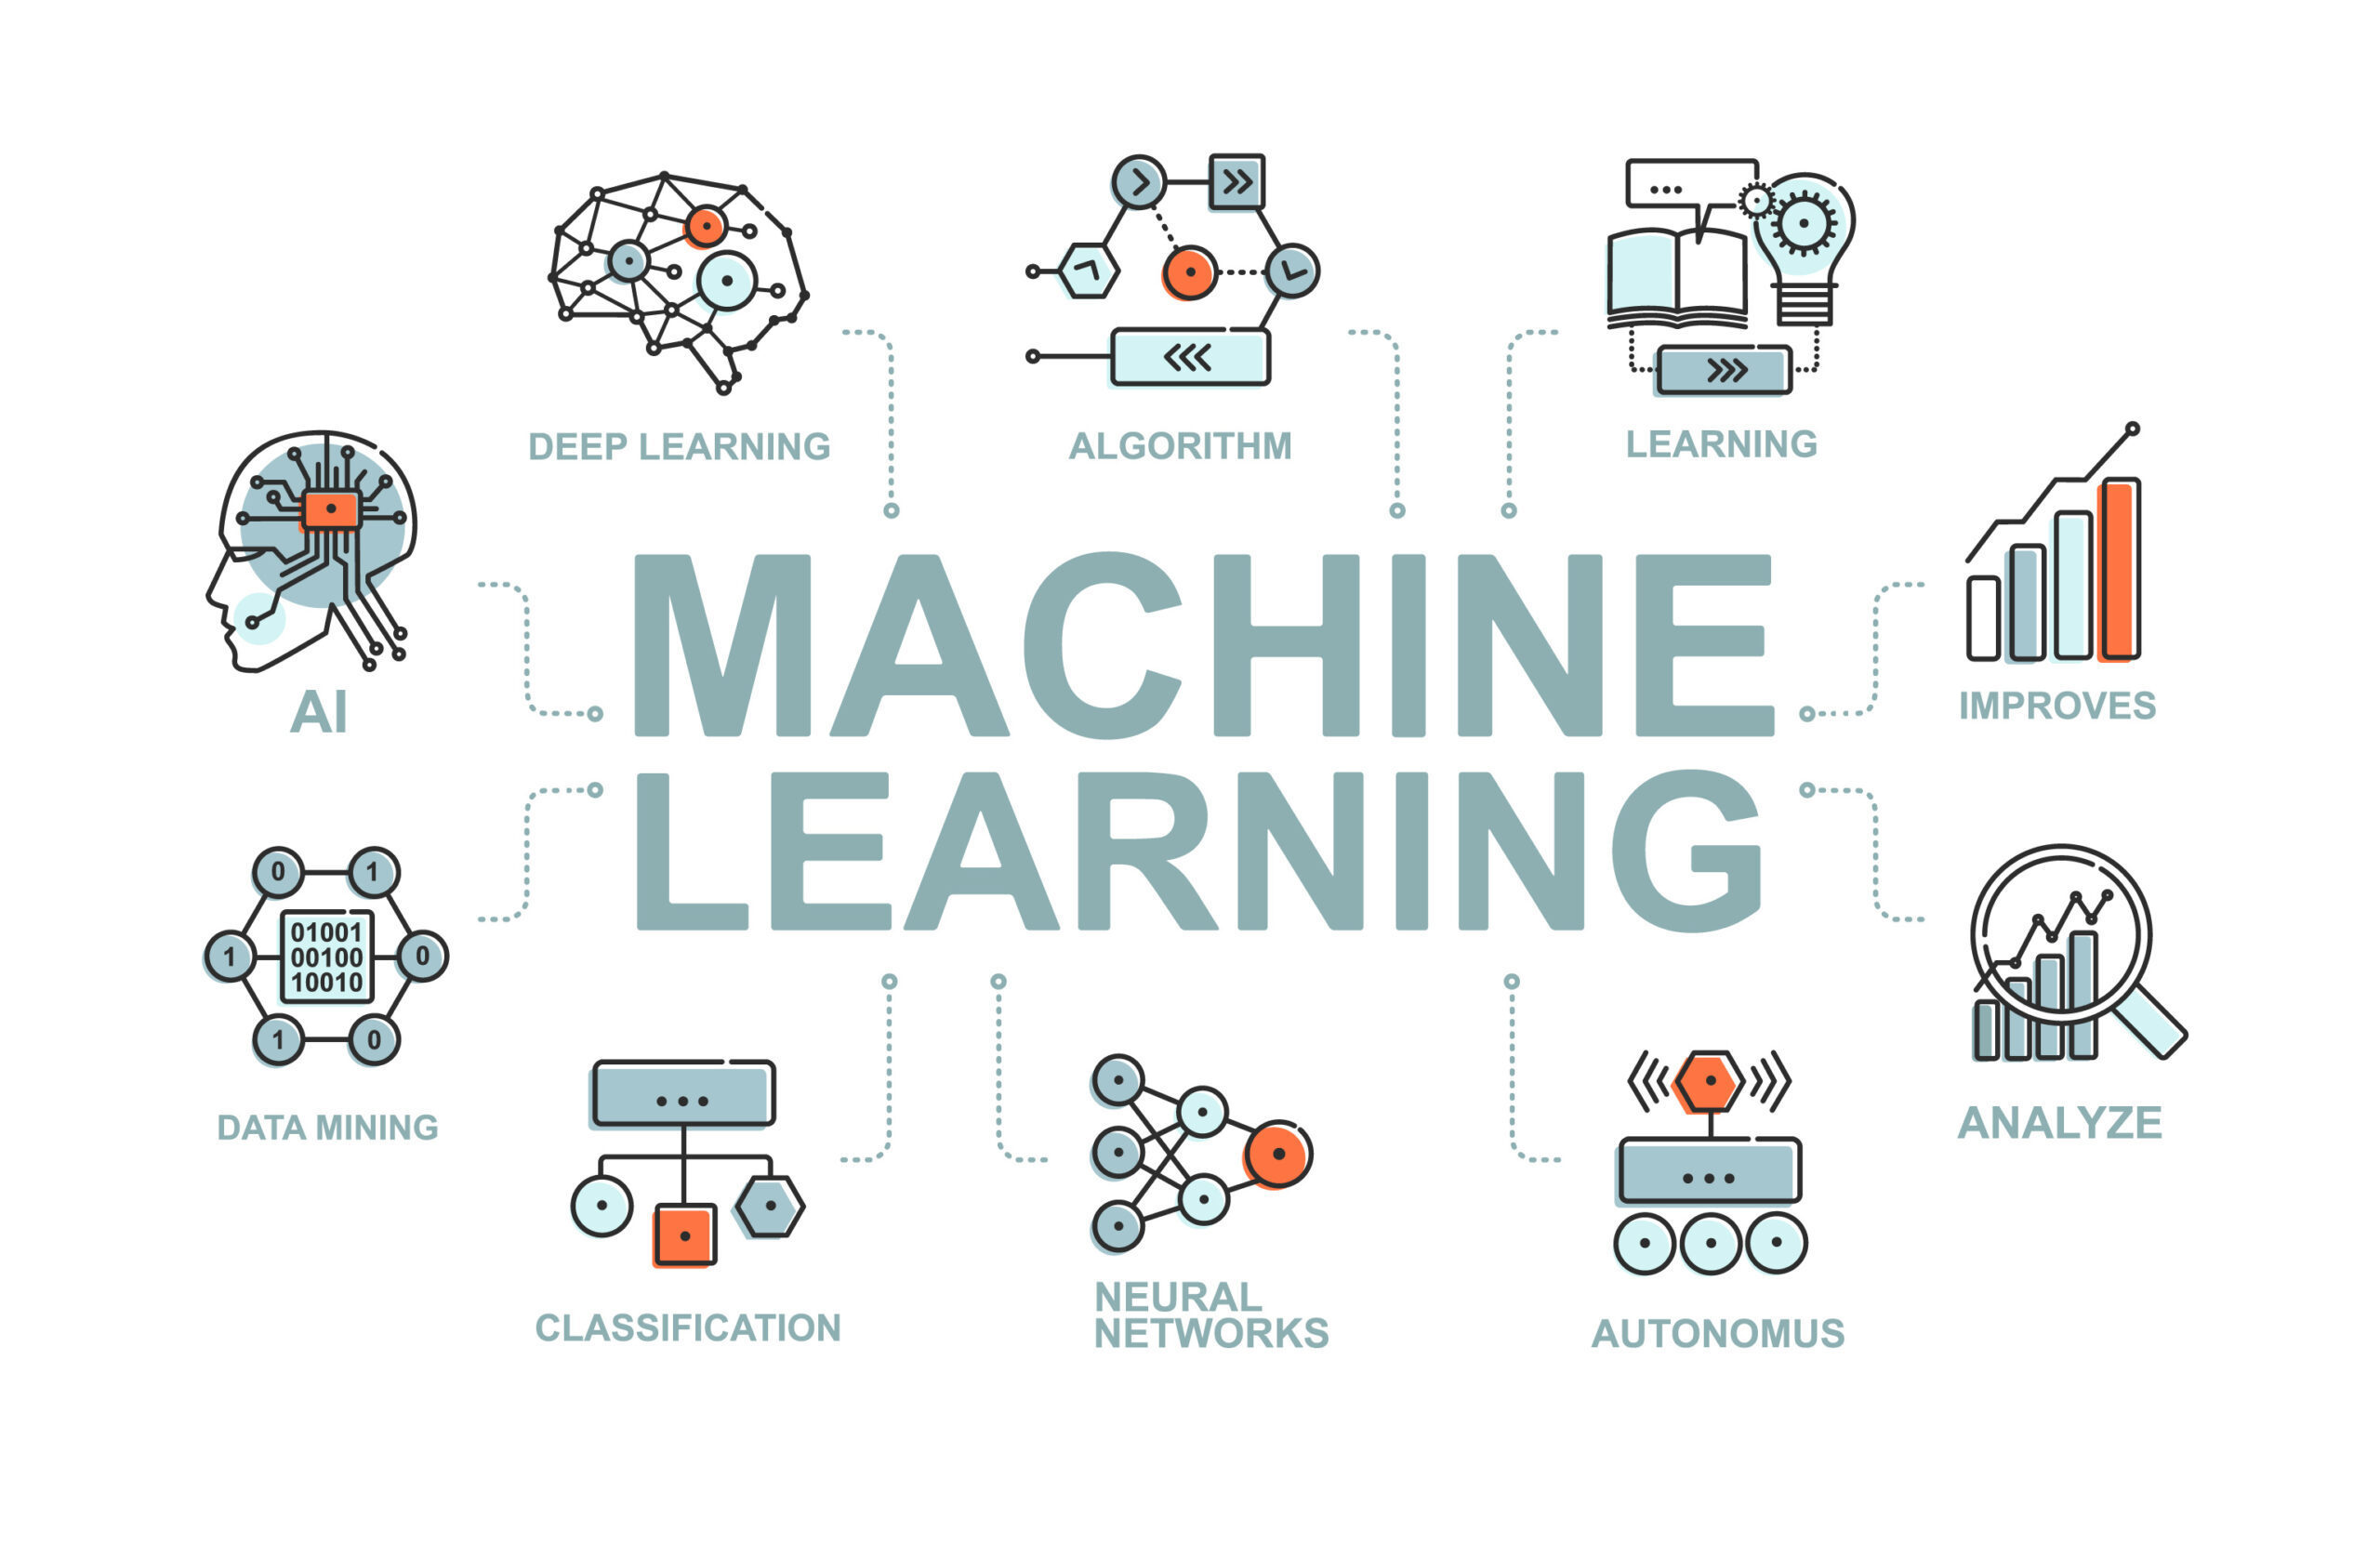
\includegraphics[width=0.5\linewidth]{images/m.jpg}
\end{center}
\vspace{1cm}
%Supervisor's Details
\begin{center}
    {\Large Data Science 871: Machine Learning Project\par}
    \vspace{1cm}
%Degree
    {\large \par}
    \vspace{1cm}
%Institution
    {\large \par}
    \vspace{1cm}
%Date
    {\large }
%More
    {\normalsize }
%More
    {\normalsize }
\end{center}
\end{minipage}
\end{center}
\clearpage


\begin{frontmatter}  %

\title{}

% Set to FALSE if wanting to remove title (for submission)


\vspace{1cm}





\vspace{0.5cm}

\end{frontmatter}


\renewcommand{\contentsname}{Table of Contents}
{\tableofcontents}

%________________________
% Header and Footers
%%%%%%%%%%%%%%%%%%%%%%%%%%%%%%%%%
\pagestyle{fancy}
\chead{}
\rhead{}
\lfoot{}
\rfoot{\footnotesize Page \thepage}
\lhead{}
%\rfoot{\footnotesize Page \thepage } % "e.g. Page 2"
\cfoot{}

%\setlength\headheight{30pt}
%%%%%%%%%%%%%%%%%%%%%%%%%%%%%%%%%
%________________________

\headsep 35pt % So that header does not go over title




\newpage

\hypertarget{introduction}{%
\section{\texorpdfstring{Introduction
\label{Introduction}}{Introduction }}\label{introduction}}

Machine learning is a field that develops algorithms designed to be
applied to data sets, usually with the goal of prediction,
classification, and clustering (\protect\hyperlink{ref-eco}{Athey}
(\protect\hyperlink{ref-eco}{2019})). Given that economists often work
with data (mostly using econometrics and statistical modeling), machine
learning could be a valuable addition to the economic toolkit. One of
the advantages of machine learning algorithms is that they can handle
large data sets that are multi-dimensional and multi-variety. With there
being a significant increase in data availability for economics and
other fields, machine learning offers researchers a method to process
and exploit large volumes of data more efficiently than traditional
statistical methods (\protect\hyperlink{ref-ecoml}{Storm, Baylis \&
Heckelei} (\protect\hyperlink{ref-ecoml}{2019})). Machine learning also
offers economists the opportunity to build more flexible models, which
is useful since economic theory is often vague about the specific
functional forms of objects to be estimated.

While linear regression analysis is commonly used in labour economics to
decompose wages, it would be interesting to see if other machine
learning algorithms could provide insight on such analysis. This paper
therefore investigates how well machine learning techniques can predict
income, given certain predictive variables. The second part of the paper
explores how well race can be predicted using machine learning. The
focus of this essay is on executing machine learning algorithms and
demonstrating the use of SQL tools, rather than the economic
interpretation of the model results. I include some discussion of the
code used to generate the results as well as some of the intuition
behind the machine learning methods.

This paper\footnote{This assignment was written using the package by
  \protect\hyperlink{ref-Texevier}{Katzke}
  (\protect\hyperlink{ref-Texevier}{2017})} is structured as follows.
First, the data set - NIDS - is discussed in section \ref{Data}. Then
the methodology is explained in section \ref{Meth}, which focuses on the
use of SQL. Section \ref{ML} applies machine learning techniques to the
NIDS data set, and comprises two subsections. The first subsection
(\ref{income}) compares the effectiveness of linear regression and
regularized regression on predicting people's incomes. The second
subsection (\ref{race}) evaluates 5 classification algorithms - Linear
Discriminant Analysis, Classification and Regression Trees, k-Nearest
Neighbors, Support Vector Machines with a linear kernel and Random
Forest - on their accuracy in predicting a person's race. The final
section (\ref{con}) concludes\footnote{This project can be found on
  Github at \url{https://github.com/cass-code/Machine-Learning.git}}.

\hypertarget{data}{%
\section{\texorpdfstring{Data \label{Data}}{Data }}\label{data}}

The data used for this assignment was sourced from the National Income
Dynamics Survey (NIDS) (\protect\hyperlink{ref-nids}{\emph{National
income dynamics study 2017, wave 5 dataset}}
(\protect\hyperlink{ref-nids}{2018})). The survey is a nationally
representative household panel study, which started in 2008 with a group
of over 28,000 individuals from 7,300 households. The same households
are surveyed every 2 years for NIDS. The latest survey - wave 5 - was
conducted in 2017. For wave 5, a total of 39,434 individuals were
interviewed; 20,113 of which were part of the original study - wave 1 -
and 2,016 were from a top-up sample. NIDS is funded by the Department of
Planning, Monitoring and Evaluation and the survey is implemented by the
Southern Africa Labour and Development Research Unit (SALDRU) at the
University of Cape Town. The data set is comprehensive and covers topics
relating to poverty, health, household composition, mortality,
expenditure, income and employment. The NIDS data set is partitioned
into different units of observations (e.g.~adults, children, household
etc.); for the machine learning component of this assignment, data from
wave 5 was used, with adults as the unit of observation.

One weakness of the NIDS data set is that it suffers from the common
problem that households at the higher end of the income distribution
tend to be underrepresented. This could be explained by the fact that
the rich refuse to fill out forms or they underreport their incomes.
Because race and income are highly correlated in South Africa, this
could also imply that white people are undersampled.

\hypertarget{methodology}{%
\section{\texorpdfstring{Methodology
\label{Meth}}{Methodology }}\label{methodology}}

Before exploring the data, I first put it into a relational database.
Relational databases are useful because they organize data into tables
which can be linked based on data common to each. This allows for
entirely new tables to be fetched/created from data in one or more
tables with a single query. To communicate with the relational database,
I used Structured Query Language (SQL) via SQLite.\footnote{I found I
  struggle quite a bit using SQL but it has got easier with practice.}
To start investigating and visualising the data, I first ran the code in
the R script called SQL. I opened a new connection and called it nids,
and wrote the NIDS data, which included waves 2-5, into tables in the
NIDS database. I used a few lines of code to check what tables were in
nids and what their source was. Then I started to explore the NIDS wave
5 data, for example, looking at the column names. I queried the data and
selected 7 variables for analysis: date of birth, income, gender,
marital status, race, years of schooling and tertiary qualification. I
used date of birth to calculate the variable `age'.

I cleaned the data by renaming the variables to be reader-friendly and
removed values that were nonsensical (e.g.~negative years of schooling)
by applying filters to the data. I wanted to see the proportion of the
races so I first manipulated the data in the SQL script and then used
the function `show\_query' to get the code for SQL. I copied this into
the r chunk in the markdown file and then graphed the results using
ggplot2. The code below shows some of this process and output:

\begin{Shaded}
\begin{Highlighting}[]
\FunctionTok{library}\NormalTok{(DBI)}
\NormalTok{nids }\OtherTok{\textless{}{-}}\NormalTok{ DBI}\SpecialCharTok{::}\FunctionTok{dbConnect}\NormalTok{(RSQLite}\SpecialCharTok{::}\FunctionTok{SQLite}\NormalTok{(), }\StringTok{"data/nids{-}db\textasciitilde{}output.sqlite"}\NormalTok{)}
\end{Highlighting}
\end{Shaded}

\begin{Shaded}
\begin{Highlighting}[]
\KeywordTok{SELECT}\NormalTok{ \textasciigrave{}race\textasciigrave{}, }\FunctionTok{COUNT}\NormalTok{(}\OperatorTok{*}\NormalTok{) }\KeywordTok{AS}\NormalTok{ \textasciigrave{}n\textasciigrave{}}
\KeywordTok{FROM}\NormalTok{ (}\KeywordTok{SELECT}\NormalTok{ \textasciigrave{}w5\_a\_dob\_y\textasciigrave{}, \textasciigrave{}w5\_a\_gen\textasciigrave{} }\KeywordTok{AS}\NormalTok{ \textasciigrave{}gender\textasciigrave{}, \textasciigrave{}w5\_a\_popgrp\textasciigrave{} }\KeywordTok{AS}\NormalTok{ \textasciigrave{}race\textasciigrave{}, }
\NormalTok{\textasciigrave{}w5\_a\_em1pay\textasciigrave{} }\KeywordTok{AS}\NormalTok{ \textasciigrave{}income\textasciigrave{}, \textasciigrave{}w5\_a\_mar\textasciigrave{} }\KeywordTok{AS}\NormalTok{ \textasciigrave{}married\textasciigrave{}, \textasciigrave{}w5\_a\_edschgrd\textasciigrave{} }\KeywordTok{AS}\NormalTok{ \textasciigrave{}school\textasciigrave{}, }
\NormalTok{\textasciigrave{}w5\_a\_edter\textasciigrave{} }\KeywordTok{AS}\NormalTok{ \textasciigrave{}tertiary\textasciigrave{} }\KeywordTok{FROM}\NormalTok{ \textasciigrave{}wave5\textasciigrave{}) }\KeywordTok{WHERE}\NormalTok{ (\textasciigrave{}race\textasciigrave{} }\OperatorTok{\textgreater{}} \FloatTok{0.0} \KeywordTok{AND}\NormalTok{ \textasciigrave{}race\textasciigrave{} }\OperatorTok{\textless{}} \FloatTok{5.0}\NormalTok{)}
\KeywordTok{GROUP} \KeywordTok{BY}\NormalTok{ \textasciigrave{}race\textasciigrave{}}
\end{Highlighting}
\end{Shaded}

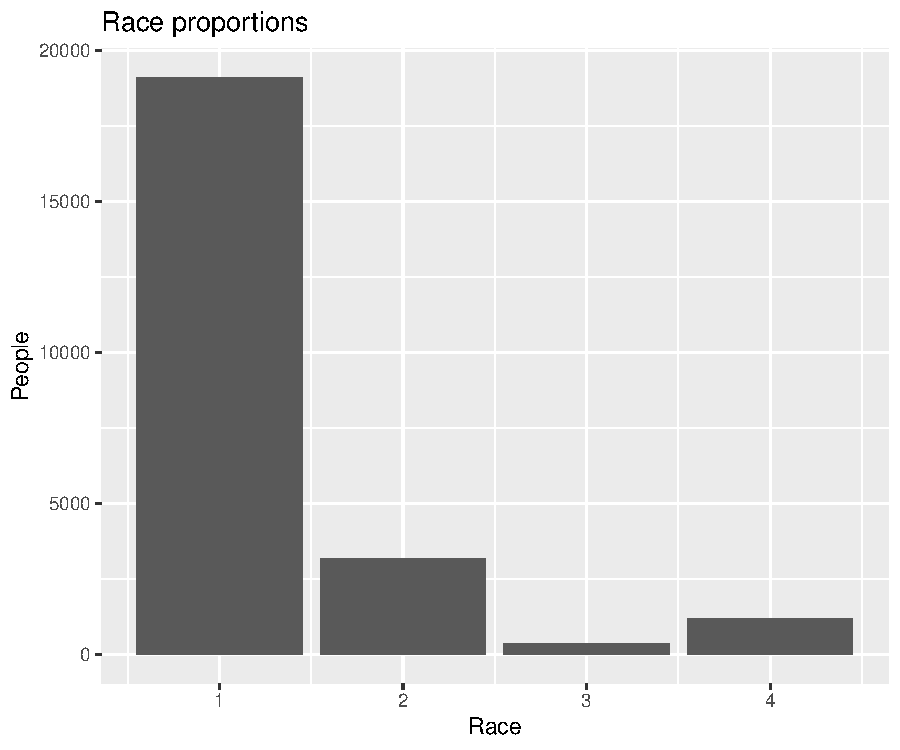
\includegraphics{20346212MLProject_files/figure-latex/unnamed-chunk-3-1.pdf}

\begin{tabular}{l}
\hline
Race\\
\hline
1 = African\\
\hline
2 = Coloured\\
\hline
3 = Asian/Indian\\
\hline
4 = White\\
\hline
\end{tabular}

The bar graph above shows that the majority of people sampled are
African and the smallest proportion are Asian/Indian. In general the
proportions appear to match the race distribution of the South African
population. The histogram below reports the number of years of
schooling. We can see that the majority of the sample has had 12 years
of schooling. The data for this graph was also manipulated using the SQL
script and then the SQL code was copied into the r chunk.

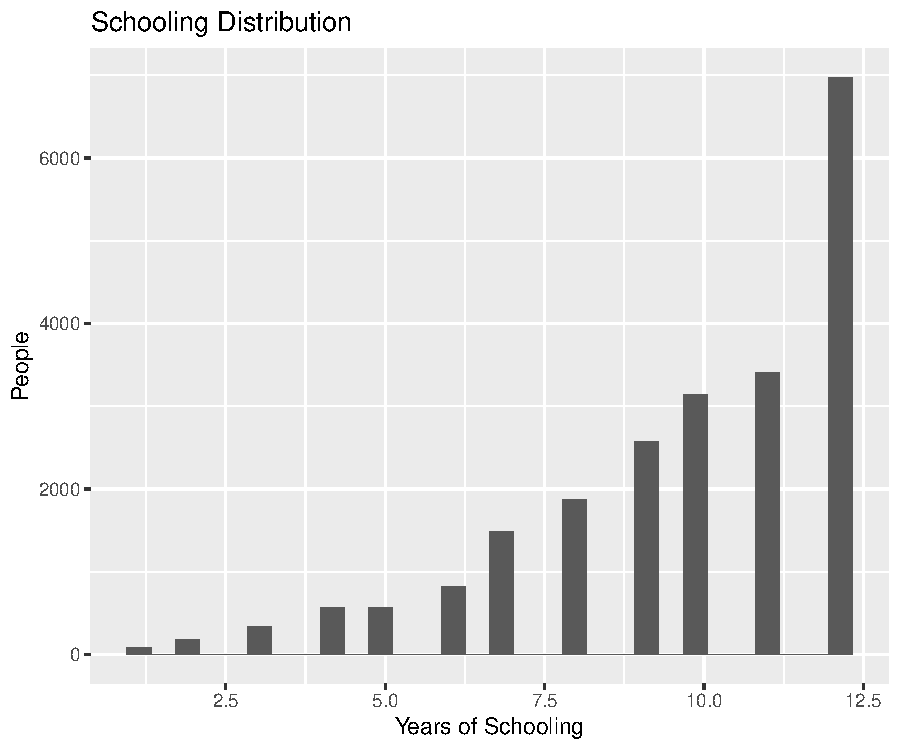
\includegraphics{20346212MLProject_files/figure-latex/unnamed-chunk-5-1.pdf}

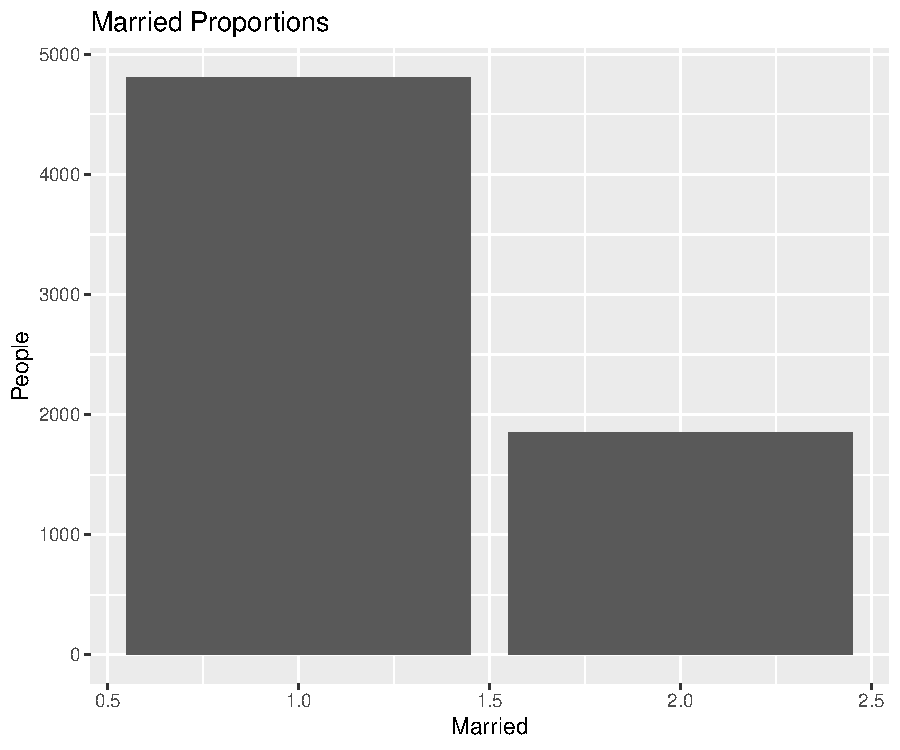
\includegraphics{20346212MLProject_files/figure-latex/unnamed-chunk-7-1.pdf}

\begin{tabular}{l}
\hline
Married\\
\hline
1 = Married\\
\hline
2 = Not married\\
\hline
\end{tabular}

Looking at the graph above, we see the proportion of people who are
married versus those that are not; clearly there are more people married
than unmarried in this sample.

If I had wanted to use more than one of the NIDS data sets, say wave 4
and 5, I could merge the two data sets using the SQL code below. I
lightly cleaned both data sets beforehand and then used the union\_all
function to merge them.

\begin{Shaded}
\begin{Highlighting}[]
\KeywordTok{SELECT} \FloatTok{2021.0} \OperatorTok{{-}}\NormalTok{ \textasciigrave{}w5\_a\_dob\_y\textasciigrave{} }\KeywordTok{AS}\NormalTok{ \textasciigrave{}age\textasciigrave{}, \textasciigrave{}w5\_a\_gen\textasciigrave{} }\KeywordTok{AS}\NormalTok{ \textasciigrave{}gender\textasciigrave{}, }
\NormalTok{\textasciigrave{}w5\_a\_popgrp\textasciigrave{} }\KeywordTok{AS}\NormalTok{ \textasciigrave{}race\textasciigrave{}, \textasciigrave{}w5\_a\_em1pay\textasciigrave{} }\KeywordTok{AS}\NormalTok{ \textasciigrave{}income\textasciigrave{}, }
\NormalTok{\textasciigrave{}w5\_a\_mar\textasciigrave{} }\KeywordTok{AS}\NormalTok{ \textasciigrave{}married\textasciigrave{}, \textasciigrave{}w5\_a\_edschgrd\textasciigrave{} }\KeywordTok{AS}\NormalTok{ \textasciigrave{}school\textasciigrave{}, }
\NormalTok{\textasciigrave{}w5\_a\_edter\textasciigrave{} }\KeywordTok{AS}\NormalTok{ \textasciigrave{}tertiary\textasciigrave{} }\KeywordTok{FROM}\NormalTok{ \textasciigrave{}wave5\textasciigrave{}}
\KeywordTok{UNION} \KeywordTok{ALL}
\KeywordTok{SELECT} \FloatTok{2021.0} \OperatorTok{{-}}\NormalTok{ \textasciigrave{}w4\_a\_dob\_y\textasciigrave{} }\KeywordTok{AS}\NormalTok{ \textasciigrave{}age\textasciigrave{}, \textasciigrave{}w4\_a\_gen\textasciigrave{} }\KeywordTok{AS}\NormalTok{ \textasciigrave{}gender\textasciigrave{}, }
\NormalTok{\textasciigrave{}w4\_a\_popgrp\textasciigrave{} }\KeywordTok{AS}\NormalTok{ \textasciigrave{}race\textasciigrave{}, \textasciigrave{}w4\_a\_em1pay\textasciigrave{} }\KeywordTok{AS}\NormalTok{ \textasciigrave{}income\textasciigrave{}, }
\NormalTok{\textasciigrave{}w4\_a\_mar\textasciigrave{} }\KeywordTok{AS}\NormalTok{ \textasciigrave{}married\textasciigrave{}, \textasciigrave{}w4\_a\_edschgrd\textasciigrave{} }\KeywordTok{AS}\NormalTok{ \textasciigrave{}school\textasciigrave{}, }
\NormalTok{\textasciigrave{}w4\_a\_edter\textasciigrave{} }\KeywordTok{AS}\NormalTok{ \textasciigrave{}tertiary\textasciigrave{} }\KeywordTok{FROM}\NormalTok{ \textasciigrave{}wave4\textasciigrave{}}
\end{Highlighting}
\end{Shaded}

The table below provides a glimpse into the first 5 rows of the newly
joined data set. I output a variable in the previous chunk as a
dataframe and then displayed the dataframe in a table in the next r
chunk. However, I could have used the function `head' in the SQL script
on the joined dataframe and the used the `collect()' function to save
the output to a global object and then displayed that object as a
dataframe.

\begin{tabular}{r|r|r|r|r|r|r}
\hline
age & gender & race & income & married & school & tertiary\\
\hline
41 & 1 & 2 & 23752 & 1 & 12 & 1\\
\hline
28 & 1 & 1 & NA & NA & 10 & 2\\
\hline
42 & 2 & 1 & NA & 1 & 11 & 1\\
\hline
49 & 1 & 1 & NA & 1 & 11 & 1\\
\hline
54 & 1 & 1 & NA & NA & 25 & NA\\
\hline
\end{tabular}

After the initial data exploration I decided to focus on predicting
income and race using machine learning techniques, which are presented
in the following section.

\hypertarget{machine-learning}{%
\section{\texorpdfstring{Machine Learning
\label{ML}}{Machine Learning }}\label{machine-learning}}

\hypertarget{predicting-income}{%
\subsection{\texorpdfstring{Predicting Income
\label{income}}{Predicting Income }}\label{predicting-income}}

Econometrics often makes use of regression analysis to model economic
phenomena, test economic hypotheses and to forecast economic activity
\protect\hyperlink{ref-econ}{Studenmund}
(\protect\hyperlink{ref-econ}{2014: 2}). A popular method in econometric
regression modeling is that of Ordinary Least Squares; however, advances
in machine learning have presented alternative/augmenting methods that
may be (more) useful. One such augmenting method is K-fold cross
validation, which evaluates the skill of machine learning models. As
\protect\hyperlink{ref-kfold}{Rodriguez, Perez \& Lozano}
(\protect\hyperlink{ref-kfold}{2009: 569}) explain, in K-fold cross
validation, a data set is randomly split into \(k\) number of groups, of
similar sizes. The first group is considered a validation set and the
method is fitted to the other \(k-1\) groups.

Below, \ref{Regression} displays 3 different linear regressions of log
of income using K-fold cross validation. For these regressions I built a
function `linreg', which takes in a data frame, cleans and splits the
data into a training (70\% of the full data set) and a test set (30\% of
the full data set) and runs 3 different linear regressions, applying
K-fold cross validation. The sample size for the regressions amounts to
4258 observations, with the training and testing sets amounting to 2982
and 1276 respectively. The results of the regressions are then collected
and stored in a list, which is returned by the function. I use k = 10,
because empirically k=10 has been shown to have test error rate
estimates that have relatively low bias and variance
(\protect\hyperlink{ref-k}{Kassambara}
(\protect\hyperlink{ref-k}{2018a})). I have also set seed in the
function for reproducibility.

Based on the Mincerian wage equation, Regression 1 (see
\ref{Regression}) regresses log of income on age, years of schooling and
a dummy variable for if a person has a tertiary qualification or not.
Regression 2 includes a variable for age-squared and the categorical
variable race. Regression 3 includes a variable each for gender and
marriage. The signs of the coefficients of the three regressions look
fairly standard\footnote{This at least is a good indication that the
  data is fairly well cleaned and is usable for testing the machine
  learning techniques} and most of the coefficients are statistically
significant at 1\% and lower. For the variables whose coefficients are
not statistically significant, labour market literature and economic
theory suggest that they are important controls and should be included,
which justifies their presence.

 
  \providecommand{\huxb}[2]{\arrayrulecolor[RGB]{#1}\global\arrayrulewidth=#2pt}
  \providecommand{\huxvb}[2]{\color[RGB]{#1}\vrule width #2pt}
  \providecommand{\huxtpad}[1]{\rule{0pt}{#1}}
  \providecommand{\huxbpad}[1]{\rule[-#1]{0pt}{#1}}

\begin{table}[ht]
\begin{centerbox}
\begin{threeparttable}
\captionsetup{justification=centering,singlelinecheck=off}
\caption{Log-Income Regression Output}
 \label{Regression}
\setlength{\tabcolsep}{0pt}
\begin{tabular}{l l l l}


\hhline{>{\huxb{0, 0, 0}{0.8}}->{\huxb{0, 0, 0}{0.8}}->{\huxb{0, 0, 0}{0.8}}->{\huxb{0, 0, 0}{0.8}}-}
\arrayrulecolor{black}

\multicolumn{1}{!{\huxvb{0, 0, 0}{0}}c!{\huxvb{0, 0, 0}{0}}}{\huxtpad{6pt + 1em}\centering \hspace{6pt} {\fontsize{12pt}{14.4pt}\selectfont } \hspace{6pt}\huxbpad{6pt}} &
\multicolumn{1}{c!{\huxvb{0, 0, 0}{0}}}{\huxtpad{6pt + 1em}\centering \hspace{6pt} {\fontsize{12pt}{14.4pt}\selectfont Reg 1} \hspace{6pt}\huxbpad{6pt}} &
\multicolumn{1}{c!{\huxvb{0, 0, 0}{0}}}{\huxtpad{6pt + 1em}\centering \hspace{6pt} {\fontsize{12pt}{14.4pt}\selectfont Reg 2} \hspace{6pt}\huxbpad{6pt}} &
\multicolumn{1}{c!{\huxvb{0, 0, 0}{0}}}{\huxtpad{6pt + 1em}\centering \hspace{6pt} {\fontsize{12pt}{14.4pt}\selectfont Reg 3} \hspace{6pt}\huxbpad{6pt}} \tabularnewline[-0.5pt]


\hhline{>{\huxb{255, 255, 255}{0.4}}->{\huxb{0, 0, 0}{0.4}}->{\huxb{0, 0, 0}{0.4}}->{\huxb{0, 0, 0}{0.4}}-}
\arrayrulecolor{black}

\multicolumn{1}{!{\huxvb{0, 0, 0}{0}}l!{\huxvb{0, 0, 0}{0}}}{\huxtpad{6pt + 1em}\raggedright \hspace{6pt} {\fontsize{12pt}{14.4pt}\selectfont (Intercept)} \hspace{6pt}\huxbpad{6pt}} &
\multicolumn{1}{r!{\huxvb{0, 0, 0}{0}}}{\huxtpad{6pt + 1em}\raggedleft \hspace{6pt} {\fontsize{12pt}{14.4pt}\selectfont 6.097 ***} \hspace{6pt}\huxbpad{6pt}} &
\multicolumn{1}{r!{\huxvb{0, 0, 0}{0}}}{\huxtpad{6pt + 1em}\raggedleft \hspace{6pt} {\fontsize{12pt}{14.4pt}\selectfont 5.791 ***} \hspace{6pt}\huxbpad{6pt}} &
\multicolumn{1}{r!{\huxvb{0, 0, 0}{0}}}{\huxtpad{6pt + 1em}\raggedleft \hspace{6pt} {\fontsize{12pt}{14.4pt}\selectfont 5.526 ***} \hspace{6pt}\huxbpad{6pt}} \tabularnewline[-0.5pt]


\hhline{}
\arrayrulecolor{black}

\multicolumn{1}{!{\huxvb{0, 0, 0}{0}}l!{\huxvb{0, 0, 0}{0}}}{\huxtpad{6pt + 1em}\raggedright \hspace{6pt} {\fontsize{12pt}{14.4pt}\selectfont } \hspace{6pt}\huxbpad{6pt}} &
\multicolumn{1}{r!{\huxvb{0, 0, 0}{0}}}{\huxtpad{6pt + 1em}\raggedleft \hspace{6pt} {\fontsize{12pt}{14.4pt}\selectfont (0.145)~~~} \hspace{6pt}\huxbpad{6pt}} &
\multicolumn{1}{r!{\huxvb{0, 0, 0}{0}}}{\huxtpad{6pt + 1em}\raggedleft \hspace{6pt} {\fontsize{12pt}{14.4pt}\selectfont (0.367)~~~} \hspace{6pt}\huxbpad{6pt}} &
\multicolumn{1}{r!{\huxvb{0, 0, 0}{0}}}{\huxtpad{6pt + 1em}\raggedleft \hspace{6pt} {\fontsize{12pt}{14.4pt}\selectfont (0.354)~~~} \hspace{6pt}\huxbpad{6pt}} \tabularnewline[-0.5pt]


\hhline{}
\arrayrulecolor{black}

\multicolumn{1}{!{\huxvb{0, 0, 0}{0}}l!{\huxvb{0, 0, 0}{0}}}{\huxtpad{6pt + 1em}\raggedright \hspace{6pt} {\fontsize{12pt}{14.4pt}\selectfont age} \hspace{6pt}\huxbpad{6pt}} &
\multicolumn{1}{r!{\huxvb{0, 0, 0}{0}}}{\huxtpad{6pt + 1em}\raggedleft \hspace{6pt} {\fontsize{12pt}{14.4pt}\selectfont 0.019 ***} \hspace{6pt}\huxbpad{6pt}} &
\multicolumn{1}{r!{\huxvb{0, 0, 0}{0}}}{\huxtpad{6pt + 1em}\raggedleft \hspace{6pt} {\fontsize{12pt}{14.4pt}\selectfont 0.041 **~} \hspace{6pt}\huxbpad{6pt}} &
\multicolumn{1}{r!{\huxvb{0, 0, 0}{0}}}{\huxtpad{6pt + 1em}\raggedleft \hspace{6pt} {\fontsize{12pt}{14.4pt}\selectfont 0.040 **~} \hspace{6pt}\huxbpad{6pt}} \tabularnewline[-0.5pt]


\hhline{}
\arrayrulecolor{black}

\multicolumn{1}{!{\huxvb{0, 0, 0}{0}}l!{\huxvb{0, 0, 0}{0}}}{\huxtpad{6pt + 1em}\raggedright \hspace{6pt} {\fontsize{12pt}{14.4pt}\selectfont } \hspace{6pt}\huxbpad{6pt}} &
\multicolumn{1}{r!{\huxvb{0, 0, 0}{0}}}{\huxtpad{6pt + 1em}\raggedleft \hspace{6pt} {\fontsize{12pt}{14.4pt}\selectfont (0.002)~~~} \hspace{6pt}\huxbpad{6pt}} &
\multicolumn{1}{r!{\huxvb{0, 0, 0}{0}}}{\huxtpad{6pt + 1em}\raggedleft \hspace{6pt} {\fontsize{12pt}{14.4pt}\selectfont (0.015)~~~} \hspace{6pt}\huxbpad{6pt}} &
\multicolumn{1}{r!{\huxvb{0, 0, 0}{0}}}{\huxtpad{6pt + 1em}\raggedleft \hspace{6pt} {\fontsize{12pt}{14.4pt}\selectfont (0.015)~~~} \hspace{6pt}\huxbpad{6pt}} \tabularnewline[-0.5pt]


\hhline{}
\arrayrulecolor{black}

\multicolumn{1}{!{\huxvb{0, 0, 0}{0}}l!{\huxvb{0, 0, 0}{0}}}{\huxtpad{6pt + 1em}\raggedright \hspace{6pt} {\fontsize{12pt}{14.4pt}\selectfont school} \hspace{6pt}\huxbpad{6pt}} &
\multicolumn{1}{r!{\huxvb{0, 0, 0}{0}}}{\huxtpad{6pt + 1em}\raggedleft \hspace{6pt} {\fontsize{12pt}{14.4pt}\selectfont 0.127 ***} \hspace{6pt}\huxbpad{6pt}} &
\multicolumn{1}{r!{\huxvb{0, 0, 0}{0}}}{\huxtpad{6pt + 1em}\raggedleft \hspace{6pt} {\fontsize{12pt}{14.4pt}\selectfont 0.109 ***} \hspace{6pt}\huxbpad{6pt}} &
\multicolumn{1}{r!{\huxvb{0, 0, 0}{0}}}{\huxtpad{6pt + 1em}\raggedleft \hspace{6pt} {\fontsize{12pt}{14.4pt}\selectfont 0.104 ***} \hspace{6pt}\huxbpad{6pt}} \tabularnewline[-0.5pt]


\hhline{}
\arrayrulecolor{black}

\multicolumn{1}{!{\huxvb{0, 0, 0}{0}}l!{\huxvb{0, 0, 0}{0}}}{\huxtpad{6pt + 1em}\raggedright \hspace{6pt} {\fontsize{12pt}{14.4pt}\selectfont } \hspace{6pt}\huxbpad{6pt}} &
\multicolumn{1}{r!{\huxvb{0, 0, 0}{0}}}{\huxtpad{6pt + 1em}\raggedleft \hspace{6pt} {\fontsize{12pt}{14.4pt}\selectfont (0.009)~~~} \hspace{6pt}\huxbpad{6pt}} &
\multicolumn{1}{r!{\huxvb{0, 0, 0}{0}}}{\huxtpad{6pt + 1em}\raggedleft \hspace{6pt} {\fontsize{12pt}{14.4pt}\selectfont (0.009)~~~} \hspace{6pt}\huxbpad{6pt}} &
\multicolumn{1}{r!{\huxvb{0, 0, 0}{0}}}{\huxtpad{6pt + 1em}\raggedleft \hspace{6pt} {\fontsize{12pt}{14.4pt}\selectfont (0.008)~~~} \hspace{6pt}\huxbpad{6pt}} \tabularnewline[-0.5pt]


\hhline{}
\arrayrulecolor{black}

\multicolumn{1}{!{\huxvb{0, 0, 0}{0}}l!{\huxvb{0, 0, 0}{0}}}{\huxtpad{6pt + 1em}\raggedright \hspace{6pt} {\fontsize{12pt}{14.4pt}\selectfont tertiary} \hspace{6pt}\huxbpad{6pt}} &
\multicolumn{1}{r!{\huxvb{0, 0, 0}{0}}}{\huxtpad{6pt + 1em}\raggedleft \hspace{6pt} {\fontsize{12pt}{14.4pt}\selectfont 0.691 ***} \hspace{6pt}\huxbpad{6pt}} &
\multicolumn{1}{r!{\huxvb{0, 0, 0}{0}}}{\huxtpad{6pt + 1em}\raggedleft \hspace{6pt} {\fontsize{12pt}{14.4pt}\selectfont 0.624 ***} \hspace{6pt}\huxbpad{6pt}} &
\multicolumn{1}{r!{\huxvb{0, 0, 0}{0}}}{\huxtpad{6pt + 1em}\raggedleft \hspace{6pt} {\fontsize{12pt}{14.4pt}\selectfont 0.594 ***} \hspace{6pt}\huxbpad{6pt}} \tabularnewline[-0.5pt]


\hhline{}
\arrayrulecolor{black}

\multicolumn{1}{!{\huxvb{0, 0, 0}{0}}l!{\huxvb{0, 0, 0}{0}}}{\huxtpad{6pt + 1em}\raggedright \hspace{6pt} {\fontsize{12pt}{14.4pt}\selectfont } \hspace{6pt}\huxbpad{6pt}} &
\multicolumn{1}{r!{\huxvb{0, 0, 0}{0}}}{\huxtpad{6pt + 1em}\raggedleft \hspace{6pt} {\fontsize{12pt}{14.4pt}\selectfont (0.048)~~~} \hspace{6pt}\huxbpad{6pt}} &
\multicolumn{1}{r!{\huxvb{0, 0, 0}{0}}}{\huxtpad{6pt + 1em}\raggedleft \hspace{6pt} {\fontsize{12pt}{14.4pt}\selectfont (0.046)~~~} \hspace{6pt}\huxbpad{6pt}} &
\multicolumn{1}{r!{\huxvb{0, 0, 0}{0}}}{\huxtpad{6pt + 1em}\raggedleft \hspace{6pt} {\fontsize{12pt}{14.4pt}\selectfont (0.044)~~~} \hspace{6pt}\huxbpad{6pt}} \tabularnewline[-0.5pt]


\hhline{}
\arrayrulecolor{black}

\multicolumn{1}{!{\huxvb{0, 0, 0}{0}}l!{\huxvb{0, 0, 0}{0}}}{\huxtpad{6pt + 1em}\raggedright \hspace{6pt} {\fontsize{12pt}{14.4pt}\selectfont age2} \hspace{6pt}\huxbpad{6pt}} &
\multicolumn{1}{r!{\huxvb{0, 0, 0}{0}}}{\huxtpad{6pt + 1em}\raggedleft \hspace{6pt} {\fontsize{12pt}{14.4pt}\selectfont ~~~~~~~~} \hspace{6pt}\huxbpad{6pt}} &
\multicolumn{1}{r!{\huxvb{0, 0, 0}{0}}}{\huxtpad{6pt + 1em}\raggedleft \hspace{6pt} {\fontsize{12pt}{14.4pt}\selectfont -0.000~~~~} \hspace{6pt}\huxbpad{6pt}} &
\multicolumn{1}{r!{\huxvb{0, 0, 0}{0}}}{\huxtpad{6pt + 1em}\raggedleft \hspace{6pt} {\fontsize{12pt}{14.4pt}\selectfont -0.000 *~~} \hspace{6pt}\huxbpad{6pt}} \tabularnewline[-0.5pt]


\hhline{}
\arrayrulecolor{black}

\multicolumn{1}{!{\huxvb{0, 0, 0}{0}}l!{\huxvb{0, 0, 0}{0}}}{\huxtpad{6pt + 1em}\raggedright \hspace{6pt} {\fontsize{12pt}{14.4pt}\selectfont } \hspace{6pt}\huxbpad{6pt}} &
\multicolumn{1}{r!{\huxvb{0, 0, 0}{0}}}{\huxtpad{6pt + 1em}\raggedleft \hspace{6pt} {\fontsize{12pt}{14.4pt}\selectfont ~~~~~~~~} \hspace{6pt}\huxbpad{6pt}} &
\multicolumn{1}{r!{\huxvb{0, 0, 0}{0}}}{\huxtpad{6pt + 1em}\raggedleft \hspace{6pt} {\fontsize{12pt}{14.4pt}\selectfont (0.000)~~~} \hspace{6pt}\huxbpad{6pt}} &
\multicolumn{1}{r!{\huxvb{0, 0, 0}{0}}}{\huxtpad{6pt + 1em}\raggedleft \hspace{6pt} {\fontsize{12pt}{14.4pt}\selectfont (0.000)~~~} \hspace{6pt}\huxbpad{6pt}} \tabularnewline[-0.5pt]


\hhline{}
\arrayrulecolor{black}

\multicolumn{1}{!{\huxvb{0, 0, 0}{0}}l!{\huxvb{0, 0, 0}{0}}}{\huxtpad{6pt + 1em}\raggedright \hspace{6pt} {\fontsize{12pt}{14.4pt}\selectfont `raceAsian/Indian`} \hspace{6pt}\huxbpad{6pt}} &
\multicolumn{1}{r!{\huxvb{0, 0, 0}{0}}}{\huxtpad{6pt + 1em}\raggedleft \hspace{6pt} {\fontsize{12pt}{14.4pt}\selectfont ~~~~~~~~} \hspace{6pt}\huxbpad{6pt}} &
\multicolumn{1}{r!{\huxvb{0, 0, 0}{0}}}{\huxtpad{6pt + 1em}\raggedleft \hspace{6pt} {\fontsize{12pt}{14.4pt}\selectfont 0.575 ***} \hspace{6pt}\huxbpad{6pt}} &
\multicolumn{1}{r!{\huxvb{0, 0, 0}{0}}}{\huxtpad{6pt + 1em}\raggedleft \hspace{6pt} {\fontsize{12pt}{14.4pt}\selectfont 0.554 ***} \hspace{6pt}\huxbpad{6pt}} \tabularnewline[-0.5pt]


\hhline{}
\arrayrulecolor{black}

\multicolumn{1}{!{\huxvb{0, 0, 0}{0}}l!{\huxvb{0, 0, 0}{0}}}{\huxtpad{6pt + 1em}\raggedright \hspace{6pt} {\fontsize{12pt}{14.4pt}\selectfont } \hspace{6pt}\huxbpad{6pt}} &
\multicolumn{1}{r!{\huxvb{0, 0, 0}{0}}}{\huxtpad{6pt + 1em}\raggedleft \hspace{6pt} {\fontsize{12pt}{14.4pt}\selectfont ~~~~~~~~} \hspace{6pt}\huxbpad{6pt}} &
\multicolumn{1}{r!{\huxvb{0, 0, 0}{0}}}{\huxtpad{6pt + 1em}\raggedleft \hspace{6pt} {\fontsize{12pt}{14.4pt}\selectfont (0.123)~~~} \hspace{6pt}\huxbpad{6pt}} &
\multicolumn{1}{r!{\huxvb{0, 0, 0}{0}}}{\huxtpad{6pt + 1em}\raggedleft \hspace{6pt} {\fontsize{12pt}{14.4pt}\selectfont (0.117)~~~} \hspace{6pt}\huxbpad{6pt}} \tabularnewline[-0.5pt]


\hhline{}
\arrayrulecolor{black}

\multicolumn{1}{!{\huxvb{0, 0, 0}{0}}l!{\huxvb{0, 0, 0}{0}}}{\huxtpad{6pt + 1em}\raggedright \hspace{6pt} {\fontsize{12pt}{14.4pt}\selectfont raceColoured} \hspace{6pt}\huxbpad{6pt}} &
\multicolumn{1}{r!{\huxvb{0, 0, 0}{0}}}{\huxtpad{6pt + 1em}\raggedleft \hspace{6pt} {\fontsize{12pt}{14.4pt}\selectfont ~~~~~~~~} \hspace{6pt}\huxbpad{6pt}} &
\multicolumn{1}{r!{\huxvb{0, 0, 0}{0}}}{\huxtpad{6pt + 1em}\raggedleft \hspace{6pt} {\fontsize{12pt}{14.4pt}\selectfont 0.023~~~~} \hspace{6pt}\huxbpad{6pt}} &
\multicolumn{1}{r!{\huxvb{0, 0, 0}{0}}}{\huxtpad{6pt + 1em}\raggedleft \hspace{6pt} {\fontsize{12pt}{14.4pt}\selectfont 0.008~~~~} \hspace{6pt}\huxbpad{6pt}} \tabularnewline[-0.5pt]


\hhline{}
\arrayrulecolor{black}

\multicolumn{1}{!{\huxvb{0, 0, 0}{0}}l!{\huxvb{0, 0, 0}{0}}}{\huxtpad{6pt + 1em}\raggedright \hspace{6pt} {\fontsize{12pt}{14.4pt}\selectfont } \hspace{6pt}\huxbpad{6pt}} &
\multicolumn{1}{r!{\huxvb{0, 0, 0}{0}}}{\huxtpad{6pt + 1em}\raggedleft \hspace{6pt} {\fontsize{12pt}{14.4pt}\selectfont ~~~~~~~~} \hspace{6pt}\huxbpad{6pt}} &
\multicolumn{1}{r!{\huxvb{0, 0, 0}{0}}}{\huxtpad{6pt + 1em}\raggedleft \hspace{6pt} {\fontsize{12pt}{14.4pt}\selectfont (0.048)~~~} \hspace{6pt}\huxbpad{6pt}} &
\multicolumn{1}{r!{\huxvb{0, 0, 0}{0}}}{\huxtpad{6pt + 1em}\raggedleft \hspace{6pt} {\fontsize{12pt}{14.4pt}\selectfont (0.046)~~~} \hspace{6pt}\huxbpad{6pt}} \tabularnewline[-0.5pt]


\hhline{}
\arrayrulecolor{black}

\multicolumn{1}{!{\huxvb{0, 0, 0}{0}}l!{\huxvb{0, 0, 0}{0}}}{\huxtpad{6pt + 1em}\raggedright \hspace{6pt} {\fontsize{12pt}{14.4pt}\selectfont raceWhite} \hspace{6pt}\huxbpad{6pt}} &
\multicolumn{1}{r!{\huxvb{0, 0, 0}{0}}}{\huxtpad{6pt + 1em}\raggedleft \hspace{6pt} {\fontsize{12pt}{14.4pt}\selectfont ~~~~~~~~} \hspace{6pt}\huxbpad{6pt}} &
\multicolumn{1}{r!{\huxvb{0, 0, 0}{0}}}{\huxtpad{6pt + 1em}\raggedleft \hspace{6pt} {\fontsize{12pt}{14.4pt}\selectfont 0.767 ***} \hspace{6pt}\huxbpad{6pt}} &
\multicolumn{1}{r!{\huxvb{0, 0, 0}{0}}}{\huxtpad{6pt + 1em}\raggedleft \hspace{6pt} {\fontsize{12pt}{14.4pt}\selectfont 0.777 ***} \hspace{6pt}\huxbpad{6pt}} \tabularnewline[-0.5pt]


\hhline{}
\arrayrulecolor{black}

\multicolumn{1}{!{\huxvb{0, 0, 0}{0}}l!{\huxvb{0, 0, 0}{0}}}{\huxtpad{6pt + 1em}\raggedright \hspace{6pt} {\fontsize{12pt}{14.4pt}\selectfont } \hspace{6pt}\huxbpad{6pt}} &
\multicolumn{1}{r!{\huxvb{0, 0, 0}{0}}}{\huxtpad{6pt + 1em}\raggedleft \hspace{6pt} {\fontsize{12pt}{14.4pt}\selectfont ~~~~~~~~} \hspace{6pt}\huxbpad{6pt}} &
\multicolumn{1}{r!{\huxvb{0, 0, 0}{0}}}{\huxtpad{6pt + 1em}\raggedleft \hspace{6pt} {\fontsize{12pt}{14.4pt}\selectfont (0.070)~~~} \hspace{6pt}\huxbpad{6pt}} &
\multicolumn{1}{r!{\huxvb{0, 0, 0}{0}}}{\huxtpad{6pt + 1em}\raggedleft \hspace{6pt} {\fontsize{12pt}{14.4pt}\selectfont (0.066)~~~} \hspace{6pt}\huxbpad{6pt}} \tabularnewline[-0.5pt]


\hhline{}
\arrayrulecolor{black}

\multicolumn{1}{!{\huxvb{0, 0, 0}{0}}l!{\huxvb{0, 0, 0}{0}}}{\huxtpad{6pt + 1em}\raggedright \hspace{6pt} {\fontsize{12pt}{14.4pt}\selectfont married} \hspace{6pt}\huxbpad{6pt}} &
\multicolumn{1}{r!{\huxvb{0, 0, 0}{0}}}{\huxtpad{6pt + 1em}\raggedleft \hspace{6pt} {\fontsize{12pt}{14.4pt}\selectfont ~~~~~~~~} \hspace{6pt}\huxbpad{6pt}} &
\multicolumn{1}{r!{\huxvb{0, 0, 0}{0}}}{\huxtpad{6pt + 1em}\raggedleft \hspace{6pt} {\fontsize{12pt}{14.4pt}\selectfont ~~~~~~~~} \hspace{6pt}\huxbpad{6pt}} &
\multicolumn{1}{r!{\huxvb{0, 0, 0}{0}}}{\huxtpad{6pt + 1em}\raggedleft \hspace{6pt} {\fontsize{12pt}{14.4pt}\selectfont 0.317 ***} \hspace{6pt}\huxbpad{6pt}} \tabularnewline[-0.5pt]


\hhline{}
\arrayrulecolor{black}

\multicolumn{1}{!{\huxvb{0, 0, 0}{0}}l!{\huxvb{0, 0, 0}{0}}}{\huxtpad{6pt + 1em}\raggedright \hspace{6pt} {\fontsize{12pt}{14.4pt}\selectfont } \hspace{6pt}\huxbpad{6pt}} &
\multicolumn{1}{r!{\huxvb{0, 0, 0}{0}}}{\huxtpad{6pt + 1em}\raggedleft \hspace{6pt} {\fontsize{12pt}{14.4pt}\selectfont ~~~~~~~~} \hspace{6pt}\huxbpad{6pt}} &
\multicolumn{1}{r!{\huxvb{0, 0, 0}{0}}}{\huxtpad{6pt + 1em}\raggedleft \hspace{6pt} {\fontsize{12pt}{14.4pt}\selectfont ~~~~~~~~} \hspace{6pt}\huxbpad{6pt}} &
\multicolumn{1}{r!{\huxvb{0, 0, 0}{0}}}{\huxtpad{6pt + 1em}\raggedleft \hspace{6pt} {\fontsize{12pt}{14.4pt}\selectfont (0.045)~~~} \hspace{6pt}\huxbpad{6pt}} \tabularnewline[-0.5pt]


\hhline{}
\arrayrulecolor{black}

\multicolumn{1}{!{\huxvb{0, 0, 0}{0}}l!{\huxvb{0, 0, 0}{0}}}{\huxtpad{6pt + 1em}\raggedright \hspace{6pt} {\fontsize{12pt}{14.4pt}\selectfont male} \hspace{6pt}\huxbpad{6pt}} &
\multicolumn{1}{r!{\huxvb{0, 0, 0}{0}}}{\huxtpad{6pt + 1em}\raggedleft \hspace{6pt} {\fontsize{12pt}{14.4pt}\selectfont ~~~~~~~~} \hspace{6pt}\huxbpad{6pt}} &
\multicolumn{1}{r!{\huxvb{0, 0, 0}{0}}}{\huxtpad{6pt + 1em}\raggedleft \hspace{6pt} {\fontsize{12pt}{14.4pt}\selectfont ~~~~~~~~} \hspace{6pt}\huxbpad{6pt}} &
\multicolumn{1}{r!{\huxvb{0, 0, 0}{0}}}{\huxtpad{6pt + 1em}\raggedleft \hspace{6pt} {\fontsize{12pt}{14.4pt}\selectfont 0.477 ***} \hspace{6pt}\huxbpad{6pt}} \tabularnewline[-0.5pt]


\hhline{}
\arrayrulecolor{black}

\multicolumn{1}{!{\huxvb{0, 0, 0}{0}}l!{\huxvb{0, 0, 0}{0}}}{\huxtpad{6pt + 1em}\raggedright \hspace{6pt} {\fontsize{12pt}{14.4pt}\selectfont } \hspace{6pt}\huxbpad{6pt}} &
\multicolumn{1}{r!{\huxvb{0, 0, 0}{0}}}{\huxtpad{6pt + 1em}\raggedleft \hspace{6pt} {\fontsize{12pt}{14.4pt}\selectfont ~~~~~~~~} \hspace{6pt}\huxbpad{6pt}} &
\multicolumn{1}{r!{\huxvb{0, 0, 0}{0}}}{\huxtpad{6pt + 1em}\raggedleft \hspace{6pt} {\fontsize{12pt}{14.4pt}\selectfont ~~~~~~~~} \hspace{6pt}\huxbpad{6pt}} &
\multicolumn{1}{r!{\huxvb{0, 0, 0}{0}}}{\huxtpad{6pt + 1em}\raggedleft \hspace{6pt} {\fontsize{12pt}{14.4pt}\selectfont (0.039)~~~} \hspace{6pt}\huxbpad{6pt}} \tabularnewline[-0.5pt]


\hhline{>{\huxb{0, 0, 0}{0.8}}->{\huxb{0, 0, 0}{0.8}}->{\huxb{0, 0, 0}{0.8}}->{\huxb{0, 0, 0}{0.8}}-}
\arrayrulecolor{black}

\multicolumn{4}{!{\huxvb{0, 0, 0}{0}}l!{\huxvb{0, 0, 0}{0}}}{\huxtpad{6pt + 1em}\raggedright \hspace{6pt} {\fontsize{12pt}{14.4pt}\selectfont  *** p $<$ 0.001;  ** p $<$ 0.01;  * p $<$ 0.05.} \hspace{6pt}\huxbpad{6pt}} \tabularnewline[-0.5pt]


\hhline{}
\arrayrulecolor{black}
\end{tabular}
\end{threeparttable}\par\end{centerbox}

\end{table}
 

Typically, economists are interested in evaluating the performance of a
model, which can be done by assessing how well the model predicts the
outcome variable. A useful statistical metric for measuring the
performance of a regression model is the Root Mean Squared Error (RMSE)
(\protect\hyperlink{ref-rmse}{Kassambara}
(\protect\hyperlink{ref-rmse}{2018b})).The RMSE measures the average
error performed by the model in predicting the outcome for an
observation. The mathematical formula for the RMSE is given by
\[RMSE = mean(\sqrt{(observeds - predicteds)^2)})\] This implies lower
the RMSE, the better the model performs.

Table \ref{Stats} reports the RMSES for both the training data and the
test data. We can see that the RMSEs decreased from regression 1 to
regression 3 for both the training and test data. This indicates that
regression 3 is a better model than both regressions 1 and 2 (and that
regression 2 has better predictive power than regression 1). The RMSEs
for the regression based on the training data are lower than for the
test data. However, the RMSEs are close enough between the two data sets
for all 3 models that the out-of-sample performance is fair; it does not
seem that any of the models have been overfitted to the training data.

\begin{table}[H]
\centering
\caption{Regression RMSEs and Observations} 
\label{Stats}
\begin{tabular}{lrr}
  \hline
Regression & RMSE Train & RMSE Test \\ 
  \hline
Reg 1 & 0.86 & 0.91 \\ 
  Reg 2 & 0.83 & 0.88 \\ 
  Reg 3 & 0.79 & 0.82 \\ 
   \hline
\end{tabular}
\end{table}

The table above shows that as more explanatory variables are added to
the regression, it appears that the model improves in predictive power.
However, it could actually be the case that the model is over fitting
the data. One method of addressing this issue is to use regularized
regression, which constrains the estimated coefficients. It does this by
introducing a penalty parameter in the objective function such that the
sum of the sum of squared errors and the penalty parameter is minimised.
Two common penalty parameters include the ridge and lasso methods.

As \protect\hyperlink{ref-ridg}{Wieringen}
(\protect\hyperlink{ref-ridg}{2021}) explains: starting with a linear
regression of the form \(Y=X \beta+\varepsilon\) we can estimate the
coefficients by ridge regression. This requires that \ref{eq1} is
solved:

\begin{align}
\hat{\beta}(\text{ridge})=\arg \min _{\beta \in \mathbb{R}^{p}} \frac{1}{n}\|Y-X \beta\|_{2}^{2}+\lambda\|\beta\|_{2}^{2} \label{eq1}
\end{align}

with \(\lambda>0\) as the regularization parameter (also known as the
tuning, penalty, or complexity parameter). Ridge regression involves
shrinking the coefficients of correlated explanatory variables equally
towards zero.

The lasso estimator requires that the optimization problem (\ref{eq2})
below is solved:

\begin{align}
\hat{\beta}(\text{lasso})=\underset{{\beta}}{\operatorname{argmin}}\|\mathbf{Y}-\mathbf{X} {\beta}\|_{2}^{2}+\lambda\|\beta\|_{1} \label{eq2}
\end{align} with \(\|\beta\|_{1}=\sum_{j=1}^{p}\left|\beta_{j}\right|\)
as the \(\ell_{1}\) -norm penalty on \(\beta\). This ensures the
sparsity principle is adhered to in the solution. Again \(\lambda\) is a
tuning parameter. For a specific \(\lambda\) value, the \(\ell_{1}\)
penalty allows the lasso to regularize the least squares fit and shrink
some components of \(\hat{\beta}\) to zero
(\protect\hyperlink{ref-lass}{Ogutu, Schulz-Streeck \& Piepho}
(\protect\hyperlink{ref-lass}{2012})). The lasso model suffers when
there is high degree of correlation among explanatory variables. The
model will arbitrarily choose one predictor and ignore the others, and
the model breaks down when all predictors are identical. The lasso
tuning parameter expects many of the coefficients to be near zero, and
only a small subset to be larger (\protect\hyperlink{ref-lass}{Ogutu,
Schulz-Streeck \& Piepho} (\protect\hyperlink{ref-lass}{2012})).

To apply the ridge and lasso methods I created two functions:
`plot\_ridge' and `plot\_lasso'. These functions use the `glmnet'
package (\protect\hyperlink{ref-glm}{Friedman, Hastie \& Tibshirani}
(\protect\hyperlink{ref-glm}{2010})) to run the regressions and return a
plot of the results, which are reported below. The tuning parameter here
is given by \(\lambda\). Initially, as \(\lambda\) increases there is a
decrease in the mean-squared error (MSE) for the lasso method, where the
first dotted line indicates the lowest MSE. For the smaller values of
lambda, this means that the lasso models has improved upon the OLS
model. In the ridge model, as \(\lambda\) increases, the coefficient
sizes are being reduced but the number of coefficients remains the same.
In the lasso model, after the log of \(\lambda\) increases to more than
-3, the number of parameters starts to decrease.

\begin{figure}
\centering
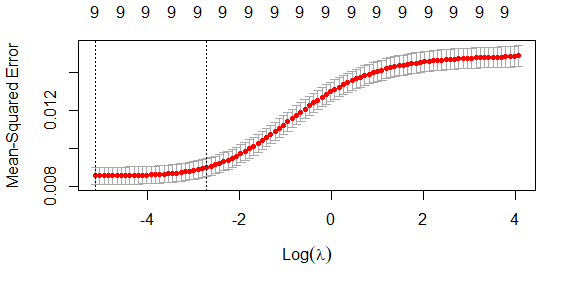
\includegraphics{"images/ridge.png"}
\caption{Ridge Model}
\end{figure}

\begin{figure}
\centering
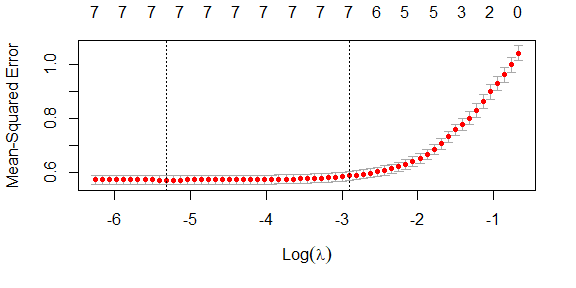
\includegraphics{"images/lasso.png"}
\caption{Lasso Model}
\end{figure}

I then created a function `comp\_RMSE', which finds the \(\lambda\) that
minimises the RMSEs for the ridge and lasso models and records the
minimised RMSEs. These models are then used to predict the log of income
for the test data. The bar chart below displays the RMSEs for the ridge
and lasso models and compares them to a base linear regression and the
three regressions from \ref{Regression}. Here, I adjusted the code from
\protect\hyperlink{ref-ridge}{Hartmann \& Waske}
(\protect\hyperlink{ref-ridge}{2018}) tutorial.

The graph shows that the RMSEs are lower for the training data than for
the test data for all the models, which could indicate the data is being
overfitted. The lasso model performs marginally better than the ridge
and linear model on the training and test sets. However, out of all the
models regression 3 performs the best on the test set, while the lasso
model performs the best on the training set. The disappointing
performance of the ridge model could be explained by the fact that there
are few predictor variables. Ridge regression performs well when there
are many explanatory variables that each have a small effect on the
outcome variable (\protect\hyperlink{ref-lass}{Ogutu, Schulz-Streeck \&
Piepho} (\protect\hyperlink{ref-lass}{2012})). We can see from the
earlier regressions that education, specifically the presence of
tertiary education, has a large effect on income, with the other
predictors having a varying degree of influence.

\begin{figure}
\centering
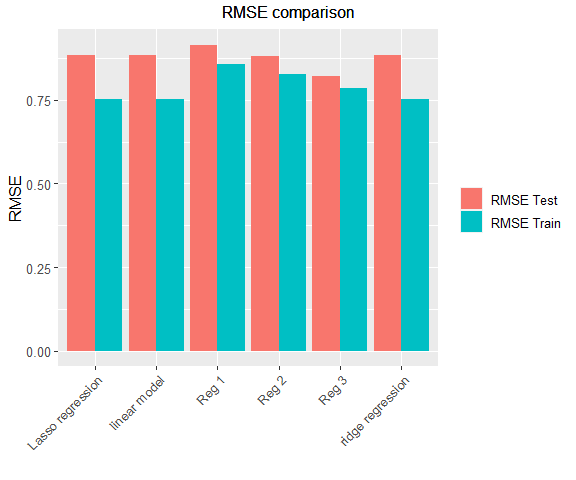
\includegraphics{"images/RMSE.png"}
\caption{RMSE comparison}
\end{figure}

While economists are interested in predicting wages based on variables
such as race and education, it might be interesting to see if race can
be predicted using income and other variables. The next section explores
this idea by applying classification algorithms on the NIDS data set.

\hypertarget{predicting-race}{%
\subsection{\texorpdfstring{Predicting Race
\label{race}}{Predicting Race }}\label{predicting-race}}

This section investigates how well race can be predicted based on
income, education, age, gender and marital status. 5 different machine
learning classification methods were implemented: Linear Discriminant
Analysis, Classification and Regression Trees, k-Nearest Neighbors,
Support Vector Machines with a linear kernel and Random Forest. Each
method is detailed below, followed by a discussion of the results of
their application to the data. Each method was applied to 3 different
data sets: first to an unbalanced data set, then to data set that was
balanced using undersampling, and finally to a data set that was
balanced using under and oversampling methods.

Linear Discriminant Analysis (LDA), is a statistical a method that finds
a linear combination of features that characterizes two or more
categories of observations. This combination can then be used as a
linear classifier. Or this combination can be used to reduce the number
of variables and dimensions of a classification problem, without there
being a significant information loss
(\protect\hyperlink{ref-lda}{Eisenbeis}
(\protect\hyperlink{ref-lda}{1971})). LDA assumes that each variable
follows a normal distribution. It also assumes that each variable has
the same variance. To make predictions, LDA estimates the likelihood
that a new set of features belongs to each group. The group that has the
highest probability is the output group and the prediction is made. To
estimate these probabilities, Bayes Theorem is used. In the figures
(\ref{fig1}, \ref{fig2}, \ref{fig3}) below, the results for the LDA
model are labeled as `lda'.

The second method used to classify the data was Classification and
Regression Trees (CART). As \protect\hyperlink{ref-cart}{Lewis}
(\protect\hyperlink{ref-cart}{2000: 4}) explains, CART analysis is a
type of binary recursive partitioning, which involves the splitting of a
node in a decision tree into two groups. Each node can be further split
into two nodes (known as child nodes), and the original node is termed a
parent node. This process can be applied several times over, hence the
``recursive'' part of binary recursive partitioning. Based on an
exhaustive search of all possibilities, CART finds ``splitting''
variables. One of the advantages of using CART is it does not make
assumptions about the underlying distribution of values of the
explanatory variables.

There are essentially four steps in the CART process. The first step
involves the tree building, where a tree is constructed via a recursive
splitting of nodes. Each of the nodes is assigned a predicted group,
based off of the distribution of groups in the training data, and the
decision cost matrix. The second step involves stopping the process of
tree building. The third step comprises tree ``pruning'', which involves
reducing the number of nodes to produce a sequence of simpler trees. The
final step is where the optimal tree is selected from the pruned trees
based on which tree fits the information of the training data without
overfitting it (\protect\hyperlink{ref-cart}{Lewis}
(\protect\hyperlink{ref-cart}{2000: 6})). The results for the CART model
are labeled as `cart' in the figures (\ref{fig1}, \ref{fig2},
\ref{fig3}) below.

The third machine learning technique is known as k-Nearest Neighbors
(KNN). As \protect\hyperlink{ref-book}{Boehmke \& Greenwell}
(\protect\hyperlink{ref-book}{2019}) explaines, KNN predicts each
observation based on how similar it is to other observations. KNN is a
supervised/memory-based machine learning algorithm. As such, it has no
closed form and when given new unlabeled data, KNN depends on labeled
input data to learn a function that produces the relevant output. One of
the disadvantages of using KNN is that it is sensitive to noisy
predictor variables since these cause similar samples to have greater
variability in distance values as well as larger magnitudes. The model
will perform poorly if there are too many outliers in the sample. The
results for the KNN model are labeled as `knn' in the charts
(\ref{fig1}, \ref{fig2}, \ref{fig3}) below.

Support Vector Machines with a linear kernel (SVM) is one of the more
advanced algorithms that is used. According to
\protect\hyperlink{ref-book}{Boehmke \& Greenwell}
(\protect\hyperlink{ref-book}{2019}), SVM aims to identify a hyperplane
in an N-dimensional space that distinctly classifies the data points.
There are many possible hyperplanes that could be chosen to partition
two groups of data points. Identifying a hyperplane that distinctly
classifies the data involves finding a plane that has the maximum
margin. Data points that lie closer to the hyperplane and influence the
orientation and position of the plane are known as support vectors.
These vectors are used to maximize the margin of the classifier and help
construct the SVM (\protect\hyperlink{ref-svm}{Gandhi}
(\protect\hyperlink{ref-svm}{2018})). The results for the SVM model are
labeled as `svm' in the figures (\ref{fig1}, \ref{fig2}, \ref{fig3})
below.

The final model used is Random Forests (RF), which is an algorithm that
comprises many decorrelated decision trees
(\protect\hyperlink{ref-book}{Boehmke \& Greenwell}
(\protect\hyperlink{ref-book}{2019})). RF generates a `forest', which is
trained by bootstrap or bagging aggregating. RF takes the average of the
predictions of the trees in the forest and uses this mean to predict
outcomes. The accuracy of the prediction can be improved by increasing
the number of trees. One advantage of using RF is that it does not
require extensive hyperparameter tuning
(\protect\hyperlink{ref-book}{Boehmke \& Greenwell}
(\protect\hyperlink{ref-book}{2019})). In the plots below (\ref{fig1},
\ref{fig2}, \ref{fig3}), the RF results are labeled as `rf'.

I built a function `ML\_plot' that applies the abovementioned algorithms
- using 10 fold cross validation where necessary - and returns a plot of
the accuracy and kappa results for each. For this, I adapted the code
from a tutorial by \protect\hyperlink{ref-ml}{Brownlee}
(\protect\hyperlink{ref-ml}{2016}). Again a split of 70\%/30\% for the
training and testing data was used. The first plot \ref{fig1} shows the
results of the algorithms on unbalanced NIDS data. The second figure
\ref{fig2} shows the results for the undersampled data and the last
figure shows the outcomes for the undersampled and oversampled data
\ref{fig3}. To balance\footnote{I originally wrote a function that
  contained the code for balancing the data. Unfortunately, calling the
  function broke my document when knitting. To get around this I
  balanced the data in an r chunk in the document, and saved the plots
  as images.} the data (i.e.~get a more equal distribution of the
different races), I used a package called ROSE by
\protect\hyperlink{ref-rose}{Lunardon, Menardi \& Torelli}
(\protect\hyperlink{ref-rose}{2014}). I first undersampled the majority
class, African; unfortunately, this method means the sample size is
reduced, which could negatively impact the prediction accuracy. To
compensate for this, I then also applied oversampling, which involves
generating more observations from the minority classes by replicating
the samples from the minority groups. The results in figure \ref{fig3}
are based on a data set where there was some undersampling of African
and some oversampling of the Coloured, Asian/Indian and White groups.

\begin{figure}[htbp]
\centering
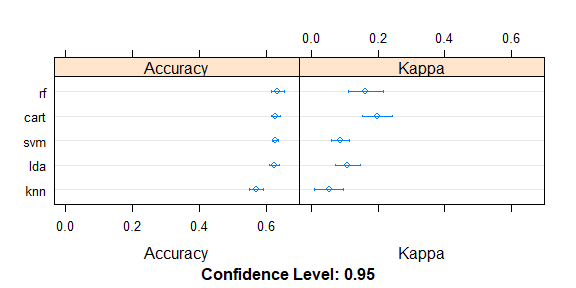
\includegraphics{images/unbal.png}
\caption{Machine Learning applied to unbalanced data \label{fig1}}
\end{figure}

\begin{figure}[htbp]
\centering
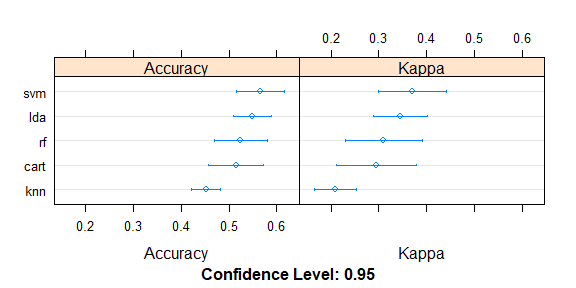
\includegraphics{images/bal1.png}
\caption{Machine Learning applied to balanced (undersampled) data \label{fig2}}
\end{figure}

\begin{figure}[htbp]
\centering
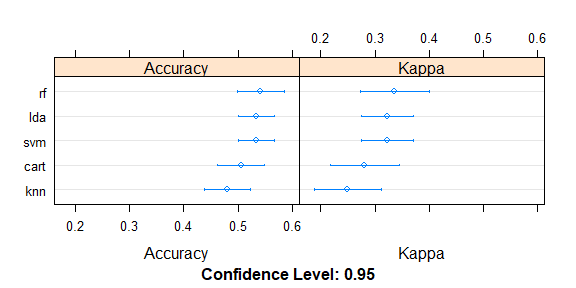
\includegraphics{images/bal2.png}
\caption{Machine Learning applied to balanced data \label{fig3}}
\end{figure}

Figure \ref{fig1} shows that the RF algorithm was (marginally) the most
accurate in predicting a person's race for the unbalanced data. It had
an accuracy measure of 62\% (using a confidence level of 95\%), where
accuracy is the ratio of the number of correct predictions to the total
number of input samples. The CART, SVM, and LDA models all performed
similarly well, with accuracy statistics lying around 60\%. The KNN
model performed the worst according to the accuracy measure. However,
accuracy isn't the only metric we should be concerned with; since the
data is unbalanced, it may be a misleading statistic. For example, since
a large part of the sample consists of the class African (let's say it's
80\%), if a model predicts African 100\% of the time, it would have an
accuracy rating of 80\%, which is not all that helpful.

A second metric we can look at is Cohen's kappa (calculated based on the
confusion matrix), which can help assess the performance of
classification models. The kappa metric accounts for an imbalance in
class distribution; this also makes it more difficult to interpret, but
a higher kappa indicates a better performing model. According to this
metric, all the models performed quite poorly. RF and CART have a
measure of around 20\% and the other models have a kappa round 10\% and
lower.

Figure \ref{fig2} reports the results of the algorithms applied to the
undersampled balanced data. We can see that the accuracy measures
decreased for all the models. This could be attributed to a smaller
sample size due to the balancing. SVM performed the best, followed by
LDA, RF, CART and KNN. Balancing the data set impacted the kappa
significantly, with all of the kappas increasing. The kappa for SVM
improved from 10\% in figure \ref{fig1} to 35\% in \ref{fig2}. Similarly
in \ref{fig3}, for the other balanced data, the kappa values for all the
models improved from those in figure \ref{fig1}. The accuracy measures
remain quite low for both balanced data sets, hovering below 60\%. The
poor predictive power of the model could be due to there being too few
predictive variables, low information predictive variables or too small
a sample size.

A more comprehensive way to gauge the performance of classification
algorithms is to look at the confusion matrix. A confusion matrix
summarizes the predictive results in a classification problem. Both
correct and incorrect predictions are tabulated with their values and
broken down by each class. The graph below (\ref{fig4}) displays the
confusion matrix for the Random Forest results on the unbalanced data
and the tables (\ref{fig5}) report the relevant statistics.

\begin{figure}[htbp]
\centering
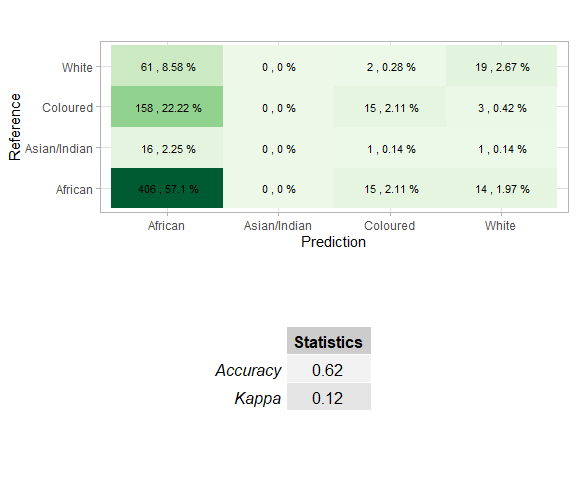
\includegraphics{images/cmrf.png}
\caption{Random Forest Confusion Matrix \label{fig4}}
\end{figure}

The y axis of figure \ref{fig4} indicates the actual values and the x
axis indicates the predicted values. The first value indicated in the
matrix show the number of predictions for that class. There are four
outcomes possible for each prediction: true positive, true negative,
false positive and false negative. The first outcome is where the model
predicted the correct class. For example, a person who is African is
predicted as African. The second outcome is that the model predicted
that a person was not of a certain race, when they were not (for
example, a person who is Coloured is not predicted as African). The
third outcome is a false positive, where a person is predicted as a
certain race when they are not. For example, a person who is White is
predicted as Asian/Indian. And finally, the fourth outcome is where a
person is predicted as not a certain race when they are. For example, a
person who is Coloured is predicted as not Coloured. The confusion
matrix and statistics measure these outcomes. For example, the bottom
left box in the confusion matrix shows the true positive for the class
African. There were 406 Africans who were correctly predicted as
African. The bottom right box in the confusion matrix shows that there
were 14 cases where a person was African but predicted as White.

The tables of \ref{fig5} detail further accuracy metrics. For example,
the sensitivity value (also known as recall) for the class Coloured is
9\%. This indicates how many cases we predicted correctly out of all the
positive classes. The fact that this value is so low indicates RF was
not successful at predicting when a person is Coloured. The model was
even worse at predicting when a person is Asian/Indian with a
specificity of 0\% - we can see why this is: the model never once
predicted that a person was Asian/Indian. Another metric we could look
at is specificity, which determines the proportion of actual negatives
that are correctly identified. For Asian/Indian this value is 100\%,
which means that for every case where a person was not Asian/Indian, the
model did not predict them to be Asian/Indian. For African, the
specificity was 15\%, which means that for 15\% of cases where a person
was not African, the model did not predict them to be African.

Precision is the ratio of the total number of correctly classified
positive classes to the total number of predicted positive classes. For
African this was 63\%, compared to 45\% for Coloured and 51\% for White.
We would like precision to be high. To help compare models that have
different precision and recall values, we can use the F-Score, which is
the harmonic mean of recall and precision. Overall, the results of the
RF are disappointing and show that the model does not have high
predictive power. It does best at correctly predicting people who are
African and very poorly at correctly predicting people who are
Asian/Indian.

\begin{figure}[htbp]
\centering
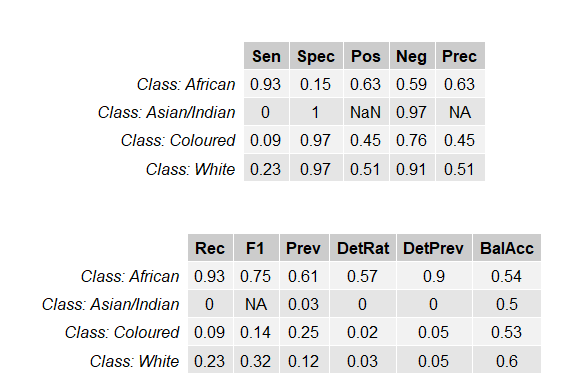
\includegraphics{images/statsrf.png}
\caption{Random Forest Statistics \label{fig5}}
\end{figure}

\hypertarget{conclusion}{%
\section{\texorpdfstring{Conclusion
\label{con}}{Conclusion }}\label{conclusion}}

The purpose of this essay was to explore machine learning techniques and
SQL tools. To this end, I manipulated the NIDS data set using SQLite and
learned how to integrate SQL and r. SQL has proven to be a powerful tool
for working with big data sets and cleaning data. In section \ref{ML},
several machine learning techniques were applied to the NIDS data set,
including linear and regularized regression as well as classification
algorithms. The results were disappointing, with the machine learning
techniques having low predictive power.

\newpage

\hypertarget{references}{%
\section*{References}\label{references}}
\addcontentsline{toc}{section}{References}

\hypertarget{refs}{}
\begin{CSLReferences}{1}{0}
\leavevmode\hypertarget{ref-eco}{}%
Athey, S. 2019. The impact of machine learning on economics. In
University of Chicago Press \emph{The economics of artificial
intelligence}. 507--552.

\leavevmode\hypertarget{ref-book}{}%
Boehmke, B. \& Greenwell, B. 2019. \emph{Hands-on machine learning with
r}.

\leavevmode\hypertarget{ref-ml}{}%
Brownlee, J. 2016. R machine learning. {[}Online{]}, Available:
\url{https://machinelearningmastery.com/machine-learning-in-r-step-by-step/}.

\leavevmode\hypertarget{ref-lda}{}%
Eisenbeis, R.A. 1971. Discriminant analysis and classification
procedures. \emph{Journal of Institutional and Theoretical Economics}.
127(3):500--521.

\leavevmode\hypertarget{ref-glm}{}%
Friedman, J., Hastie, T. \& Tibshirani, R. 2010. Regularization paths
for generalized linear models via coordinate descent. \emph{Journal of
statistical software}. 33(1):1.

\leavevmode\hypertarget{ref-svm}{}%
Gandhi, R. 2018. Support vector machine --- introduction to machine
learning algorithms. {[}Online{]}, Available:
\url{https://towardsdatascience.com/934a444fca47}.

\leavevmode\hypertarget{ref-ridge}{}%
Hartmann, K., K \& Waske, B. 2018. E-learning project SOGA: Statistics
and geospatial data analysis.

\leavevmode\hypertarget{ref-k}{}%
Kassambara, A. 2018a. Cross-validation essentials in r. {[}Online{]},
Available:
\url{http://www.sthda.com/english/articles/38-regression-model-validation/157-cross-validation-essentials-in-r/}.

\leavevmode\hypertarget{ref-rmse}{}%
Kassambara, A. 2018b. Linear regression essentials in r. {[}Online{]},
Available:
\url{http://www.sthda.com/english/articles/40-regression-analysis/165-linear-regression-essentials-in-r/}.

\leavevmode\hypertarget{ref-Texevier}{}%
Katzke, N.F. 2017. \emph{{Texevier}: {P}ackage to create elsevier
templates for rmarkdown}. Stellenbosch, South Africa: Bureau for
Economic Research.

\leavevmode\hypertarget{ref-cart}{}%
Lewis, R.J. 2000. An introduction to classification and regression tree
(CART) analysis. 14.

\leavevmode\hypertarget{ref-rose}{}%
Lunardon, N., Menardi, G. \& Torelli, N. 2014. {ROSE}: A {P}ackage for
{B}inary {I}mbalanced {L}earning. \emph{{R} Journal}. 6(1):82--92.

\leavevmode\hypertarget{ref-nids}{}%
\emph{National income dynamics study 2017, wave 5 dataset}. 2018. Cape
Town, South Africa: Department of Planning, Monitoring,; Evaluation
{[}funding agency{]} \& DataFirst {[}distributor{]}. {[}Online{]},
Available: \url{https://doi.org/10.25828/fw3h-v708}.

\leavevmode\hypertarget{ref-lass}{}%
Ogutu, J.O., Schulz-Streeck, T. \& Piepho, H.-P. 2012. Genomic selection
using regularized linear regression models: Ridge regression, lasso,
elastic net and their extensions. 6(2):1--6.

\leavevmode\hypertarget{ref-kfold}{}%
Rodriguez, J.D., Perez, A. \& Lozano, J.A. 2009. Sensitivity analysis of
k-fold cross validation in prediction error estimation. \emph{IEEE
transactions on pattern analysis and machine intelligence}.
32(3):569--575.

\leavevmode\hypertarget{ref-ecoml}{}%
Storm, H., Baylis, K. \& Heckelei, T. 2019. {Machine learning in
agricultural and applied economics}. \emph{European Review of
Agricultural Economics}. 47(3):849--892.

\leavevmode\hypertarget{ref-econ}{}%
Studenmund, A.H. 2014. \emph{Using econometrics a practical guide}.
Pearson.

\leavevmode\hypertarget{ref-ridg}{}%
Wieringen, W. van. 2021. Lecture notes on ridge regression.
{[}Online{]}, Available: \url{http://arxiv.org/abs/1509.09169}.

\end{CSLReferences}

\bibliography{Tex/ref}





\end{document}
